\section{Experimental Results}

\subsection{Baseline Performance}
The baseline models \textbf{ReLU} and \textbf{Abs} achieved strong and consistent performance on the MNIST dataset. As shown in Table~\ref{tab:baseline_performance}, ReLU exhibited a mean test accuracy of $95.64\% \pm 0.19\%$, while Abs achieved $95.26\% \pm 0.19\%$. This minimal variance across 20 runs indicates that both activation functions can effectively learn the task under standard conditions.

\begin{table}[ht]
\centering
\begin{tabular}{lcc}
\toprule
\textbf{Model} & \textbf{Test Accuracy (\%)} & \textbf{Standard Deviation (\%)} \\
\midrule
ReLU & $95.64$ & $0.19$ \\
ReLU2 & $47.20$ & $12.00$ \\
ReLU2-Neg & $94.93$ & $0.15$ \\
Abs & $95.26$ & $0.19$ \\
Abs2 & $95.35$ & $0.17$ \\
Abs2-Neg & $90.08$ & $2.56$ \\
\bottomrule
\end{tabular}
\caption{Performance metrics of all models on MNIST, including test accuracy and standard deviation.}
\label{tab:baseline_performance}
\end{table}

\subsection{Intensity Learning Models}
The models forced to learn intensity representations, through the addition of a second activation function, show significant differences in performance:
\begin{itemize}
    \item \textbf{ReLU2}: Test accuracy degraded catastrophically to $47.20\% \pm 12.00\%$. This is in line with our predictions of a distance represenation bias in the learning dynamics.
    \item \textbf{Abs2}: In contrast, Abs2 maintained robust performance at $95.35\% \pm 0.17\%$, which contradicts our prediction.
\end{itemize}

\subsection{Distance Learning Models}
The models forced to learn distance representations, which were then transformed to intensity representations with the Negative layer, also show significant differences in performance.
\begin{itemize}
    \item \textbf{ReLU2-Neg}: Performas at near-baseline levels ($94.93\% \pm 0.15\%$). The \textit{Neg} transformation enabled the network to reinterpret features as distances, mitigating instability observed in ReLU2. This supports our theory that neural networks might bias towards distance reprsentation.
    \item \textbf{Abs2-Neg}: Test accuracy dropped significantly to $90.08\% \pm 2.56\%$, with high variability between runs. While not as bad a failure as ReLU2, this result contradicts our theory that neural networks might bias towards distance representations.
\end{itemize}

\subsection{Statistical Comparisons}
T-test analysis (Table~\ref{tab:ttest_results}) shows our results are statistically significant.

\begin{table}[ht]
\centering
\begin{tabular}{lcc}
\toprule
\textbf{Comparison} & \textbf{$t$-statistic} & \textbf{$p$-value} \\
\midrule
ReLU2 vs ReLU2-Neg & $-17.33$ & $< 0.0001$ \\
Abs2 vs Abs2-Neg & $8.97$ & $< 0.0001$ \\
\bottomrule
\end{tabular}
\caption{Statistical comparisons of key model pairs.}
\label{tab:ttest_results}
\end{table}

\subsection{Training Dynamics}
The training curves reveal distinct learning patterns across architectures (Figures~\ref{fig:train_error}, \ref{fig:train_loss}, and \ref{fig:test_error}). 

\begin{figure}[ht]
\centering
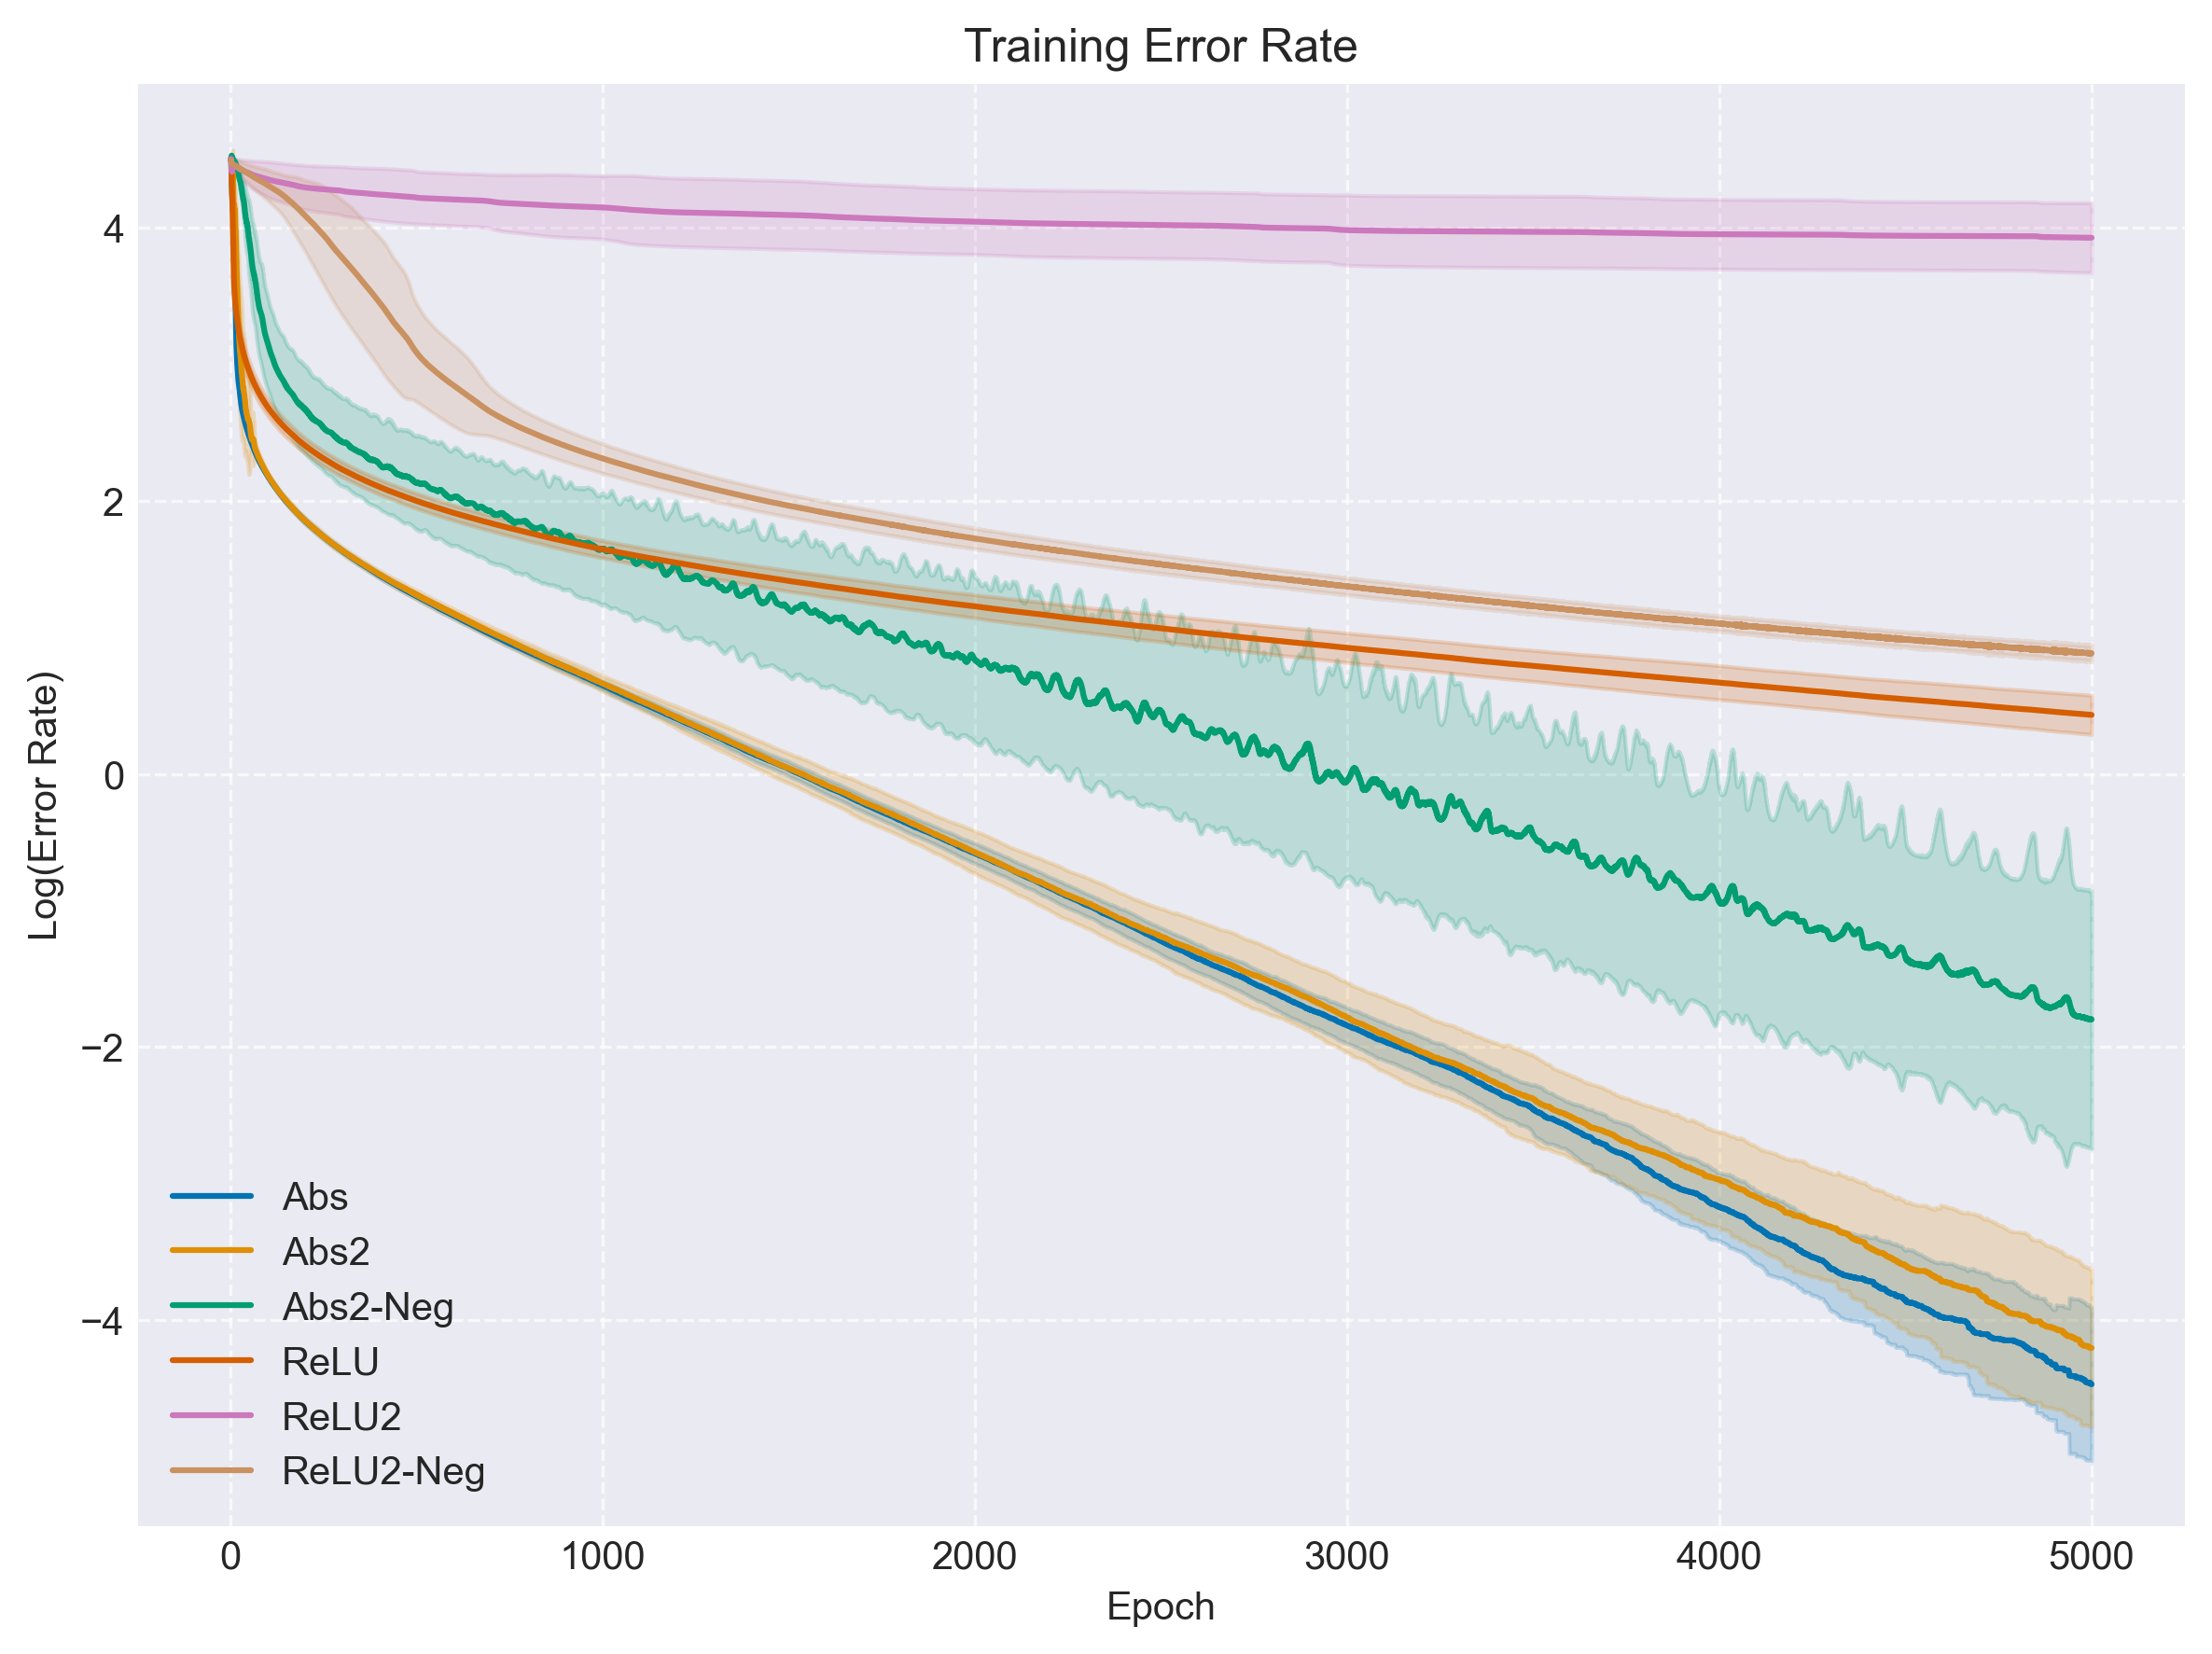
\includegraphics[width=0.8\textwidth]{images/train_error.png}
\caption{Training error rate over epochs (log scale) for all model architectures. Shaded regions represent standard deviation across 20 runs.}
\label{fig:train_error}
\end{figure}

\begin{figure}[ht]
\centering
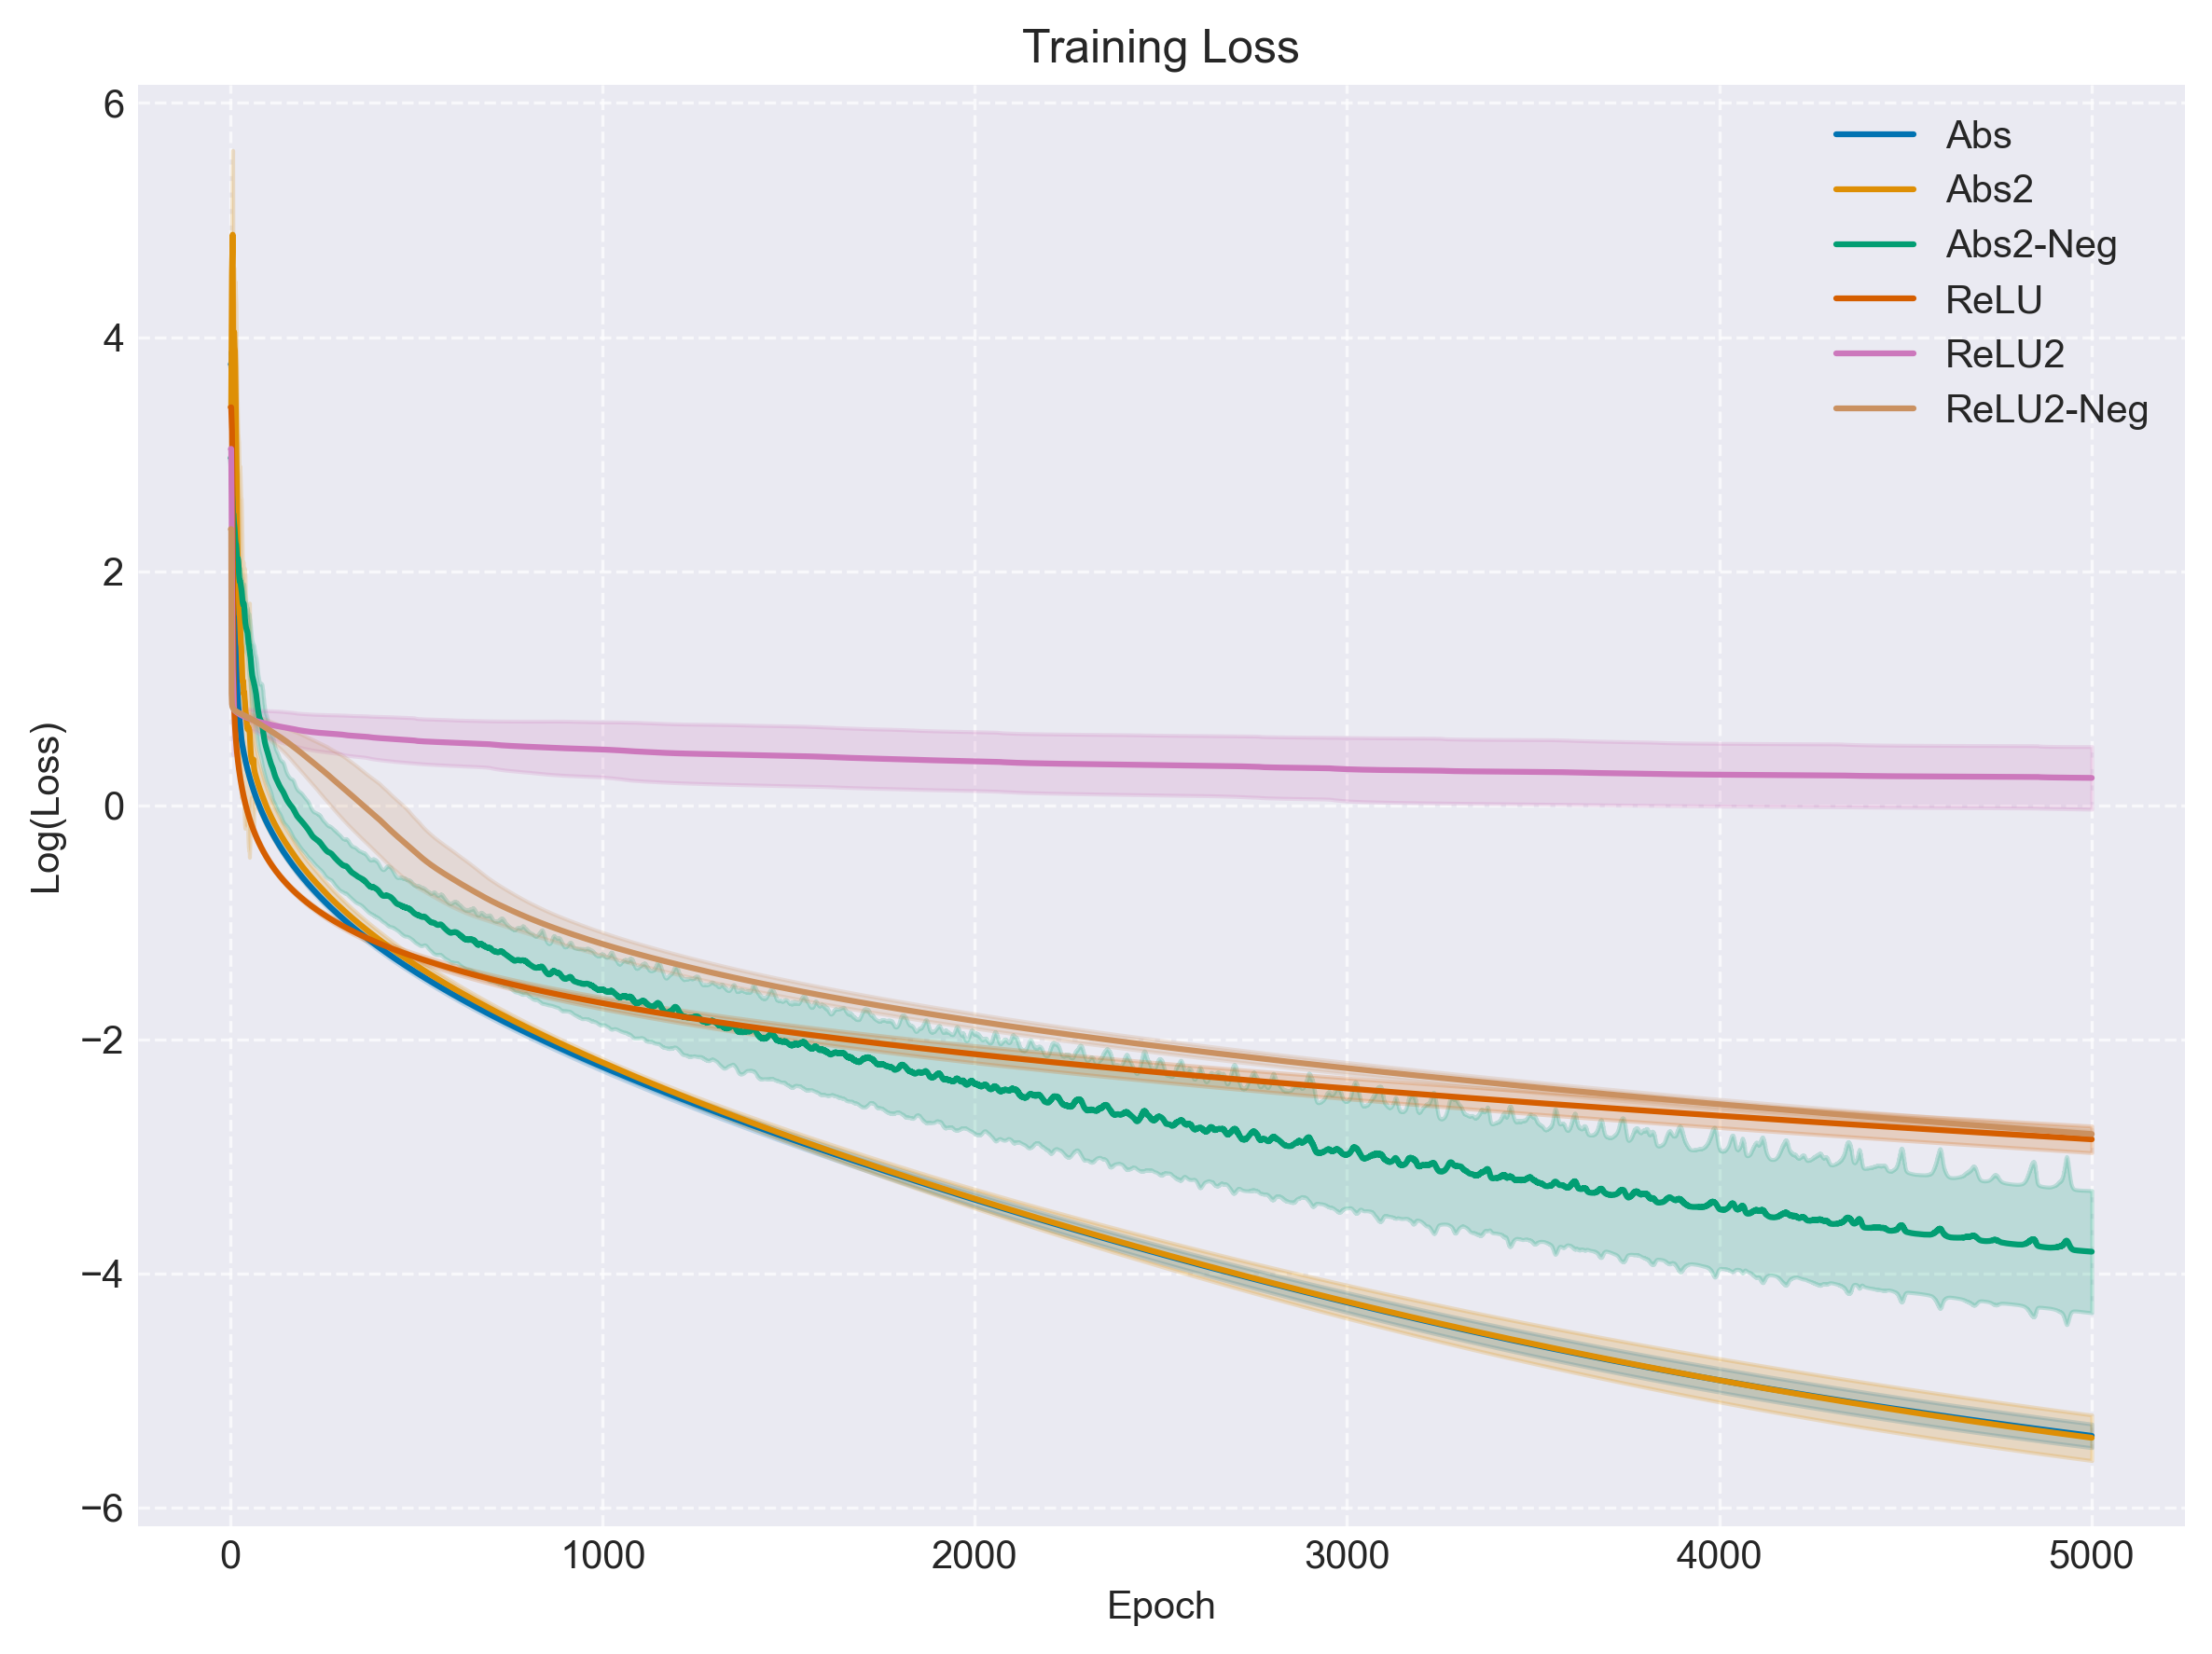
\includegraphics[width=0.8\textwidth]{images/train_loss.png}
\caption{Training loss trajectories (log scale) showing distinct convergence patterns across architectures.}
\label{fig:train_loss}
\end{figure}

\begin{figure}[ht]
\centering
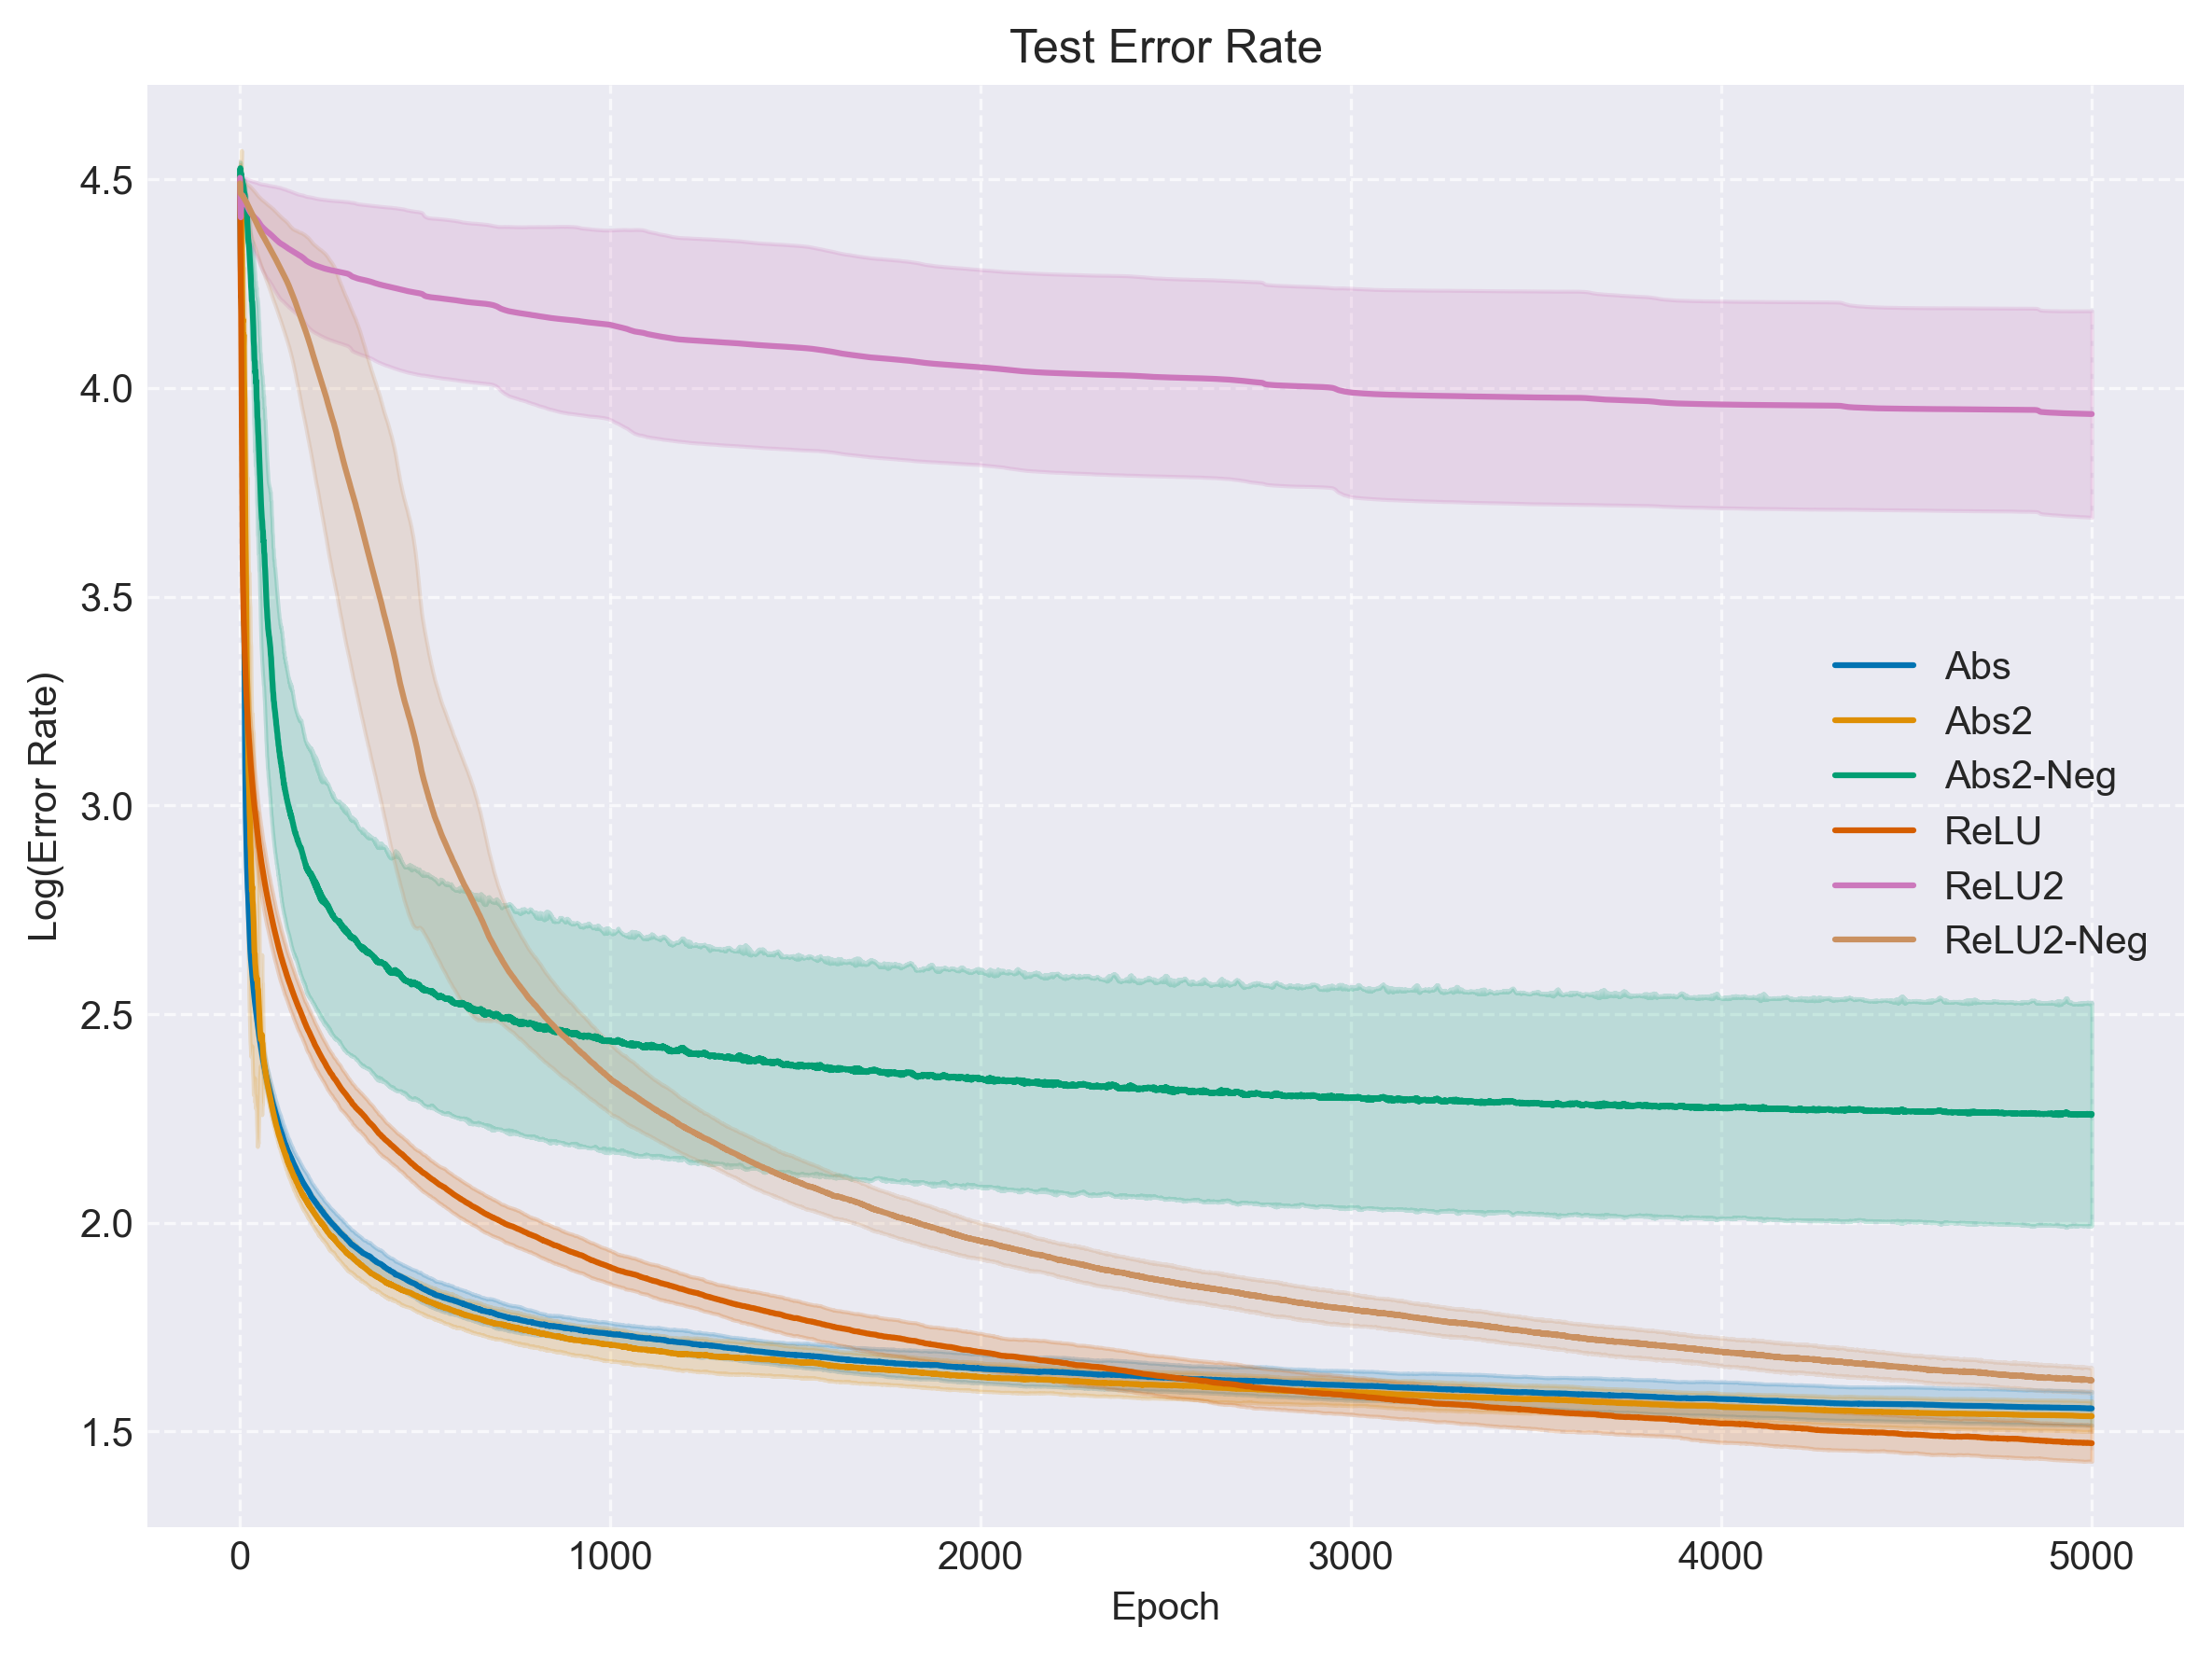
\includegraphics[width=0.8\textwidth]{images/test_error.png}
\caption{Test error rate over epochs, illustrating generalization behavior for all model architectures.}
\label{fig:test_error}
\end{figure}

\subsection{Distribution of Test Accuracies}
Figure~\ref{fig:test_dist} shows the distribution of final test accuracies across all runs, highlighting the consistency of well-performing models and the high variance in ReLU2's degraded performance. This visualization supports understanding of variance between intensity and distance representation models.

\begin{figure}[ht]
\centering
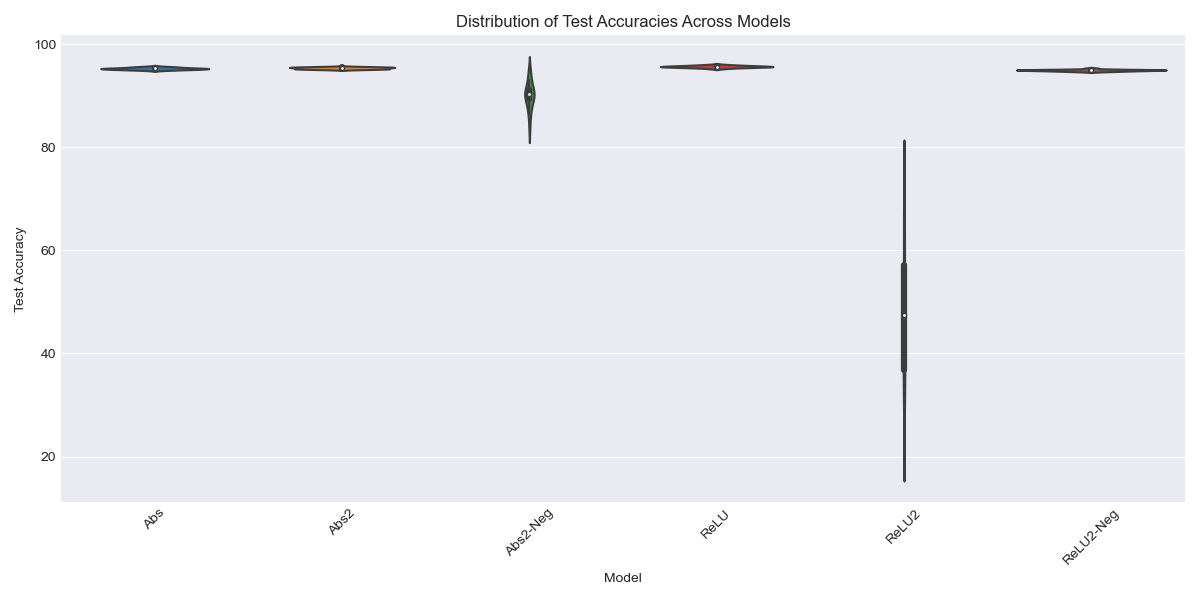
\includegraphics[width=0.8\textwidth]{images/accuracy_distribution.png}
\caption{Distribution of test accuracies across 20 runs for each architecture, showing both median performance and variance.}
\label{fig:test_dist}
\end{figure}

\subsection{Summary of Findings}

These experiments show that model performance can be affected by seemingly minor changes in architecture that control data respresentation. The results do not fully support our hypothesis that neural networks may bias towards learning distance-based representations where smaller values indicate feature acceptance.

While the ReLU2 behavior does support our theory, where catastrophic failure under intensity representations fails, but distance representation allows it to recover.

\begin{itemize}
    \item \textbf{ReLU Models}: ReLU2's catastrophic failure highlights the challenges of intensity-based representations under architectural constraints, while ReLU2-Neg demonstrates the effectiveness of \textit{Neg} transformations in restoring performance via distance distributions.
    \item \textbf{Abs Models}: Abs2 exhibited unexpected robustness, maintaining baseline performance despite theoretical predictions. Abs2-Neg revealed limitations in adapting to distance representations under combined constraints.
\end{itemize}
These findings refine our understanding of how neural networks adopt and balance distance- and intensity-based representational approaches.